\documentclass[9pt]{beamer}

\usepackage[utf8]{inputenc}
\usepackage{eurosym}
%\usepackage[francais]{babel}
%\usepackage[T1]{fontenc}
%\usepackage{url}
%\usepackage{etex}
\usepackage{enumitem}
\usepackage{multicol}
\usepackage{xcolor}
\usepackage{bbm}
\usepackage{amsmath,amsthm,amssymb}
\usepackage{pifont}
%\usepackage{exercise}
\usepackage{graphics}
\usepackage{array,multirow,makecell}
\usepackage{verbatim}
%\usepackage[dvipsnames]{pstricks}
\usepackage{pstricks-add,pst-plot,pst-text,pst-tree,pst-eps,pst-fill,pst-node,pst-math,pst-blur,pst-func}
%\usepackage{pgf,tikz}
%\usepackage{tipfr}
%\usepackage{thmbox}
\usepackage{calc}
%\usepackage{ifthen}
\usepackage{pdfpages}
%\usepackage{colortbl}
%\usepackage{sagetex}
%\usetikzlibrary{arrows,patterns}
%\input tabvar
%\usepackage{tkz-tab}
%\usepackage{listings}
%\usepackage[np]{numprint}
\usepackage{fancybox,fancyhdr}
%\usepackage{thmtools}
%\usepackage{bclogo}
%\usepackage{lastpage}

%\usepackage{tabularx}
\usepackage{array,multirow,makecell}
\usetheme{Madrid}
%\usetheme{Bergen}
\usecolortheme{beaver}
 
%Information to be included in the title page:
\title{Algorithmique}
\subtitle{Recherche dichotomique}
\author{Yannick CHISTEL}
\institute{Lycée Dumont d'Urville-CAEN}
\date{Mars 2020}
 
%----------------------------------------------------------------------------------------------- 
% 							Commandes Tableaux
%-----------------------------------------------------------------------------------------------
\setcellgapes{1pt}
\makegapedcells\newcolumntype{R}[1]{>{\raggedleft\arraybackslash}b{#1}}
\newcolumntype{L}[1]{>{\raggedright\arraybackslash}b{#1}}
\newcolumntype{C}[1]{>{\centering\arraybackslash}b{#1}}

\definecolor{vert}{rgb}{0,0,1}

\newcommand{\esp}{\hspace{0.5cm}}
\newcommand{\espp}{\hspace{1cm}}
\newcommand{\esppp}{\hspace{1.5cm}}

\newcounter{num}
\setcounter{num}{0}

\begin{document}

\frame{\titlepage}


\begin{frame}
\frametitle{Recherche dichotomique}

\begin{block}{Principe}
La \textbf{dichotomie} est un mot d'origine greque qui signifie diviser en deux.

La recherche d'une valeur dans un tableau peut être facilitée si celui-ci est trié. Dans ce cas, on divise successivement le tableau en 2 jusqu'à atteindre la valeur cherchée.
\end{block}

\begin{block}{Algorithme}
Voici une écriture de l'algorithme de recherche dichotomique dans un \textbf{tableau trié}:\\
- $t$ désigne un tableau trié\\
- $v$ est la valeur cherchée dans le tableau\\
- $a$, $b$ et $m$ sont les indices de position des valeurs dans le tableau.\medskip

$a \longleftarrow 1$\hfill\ldots\textit{première valeur du tableau}\\
$b \longleftarrow \text{longueur}(t)$\hfill\ldots\textit{dernière valeur du tableau}\\
\textbf{tant que} $a <= b$: \\
\esp$m \longleftarrow (a+b)//2 $ \hfill\ldots\textit{m est la position au milieu}\\
\esp\textbf{si} $v<t[m]$ alors $b=m-1$ \hfill\ldots\textit{v se trouve dans la première moitié}\\
\esp\textbf{sinon si} $v>t[m]$ alors $a=m+1$  \hfill\ldots\textit{v se trouve dans la seconde moitié}\\
\esp\textbf{sinon} la valeur est trouvée en $m$\\
fin \textbf{tant que}\\
La valeur n'est pas trouvée
\end{block}
\end{frame}

\begin{frame}
\frametitle{Recherche dichotomique}

Soit $T=[5,9,12,14,15,16,19,20,23,25]$ un tableau trié. On cherche le nombre 12.\medskip

\begin{minipage}{7.2cm}
\begin{enumerate}
\item $a=0$ et $b=9$: $a<b$, donc on entre dans la boucle tant que.
\item On calcule la valeur de l'indice situé au milieu du tableau: $m=(0+9)/2=4,5$ donc $m=4$. Comme $T[4]=15>12$, alors le nombre cherché est positionné avant $m$, donc $b=m-1=4-1=3$.
\item $a=0<b=3$, donc on poursuit la boucle. On calcule la valeur de $m$: $m=(0+3)/2=1,5$ donc $m=1$. Comme $T[1]=9<12$, alors le nombre cherché est positionné après $m$, donc $a=m+1=1+1=2$.
\item $a=2<b=3$, donc on poursuit la boucle. On calcule $m=(2+3)/2=2,5$ donc $m=2$. Comme $T[2]=12$, le nombre est trouvé en position $m=2$.
\end{enumerate}
\end{minipage}\hfill
\begin{minipage}{4.6cm}
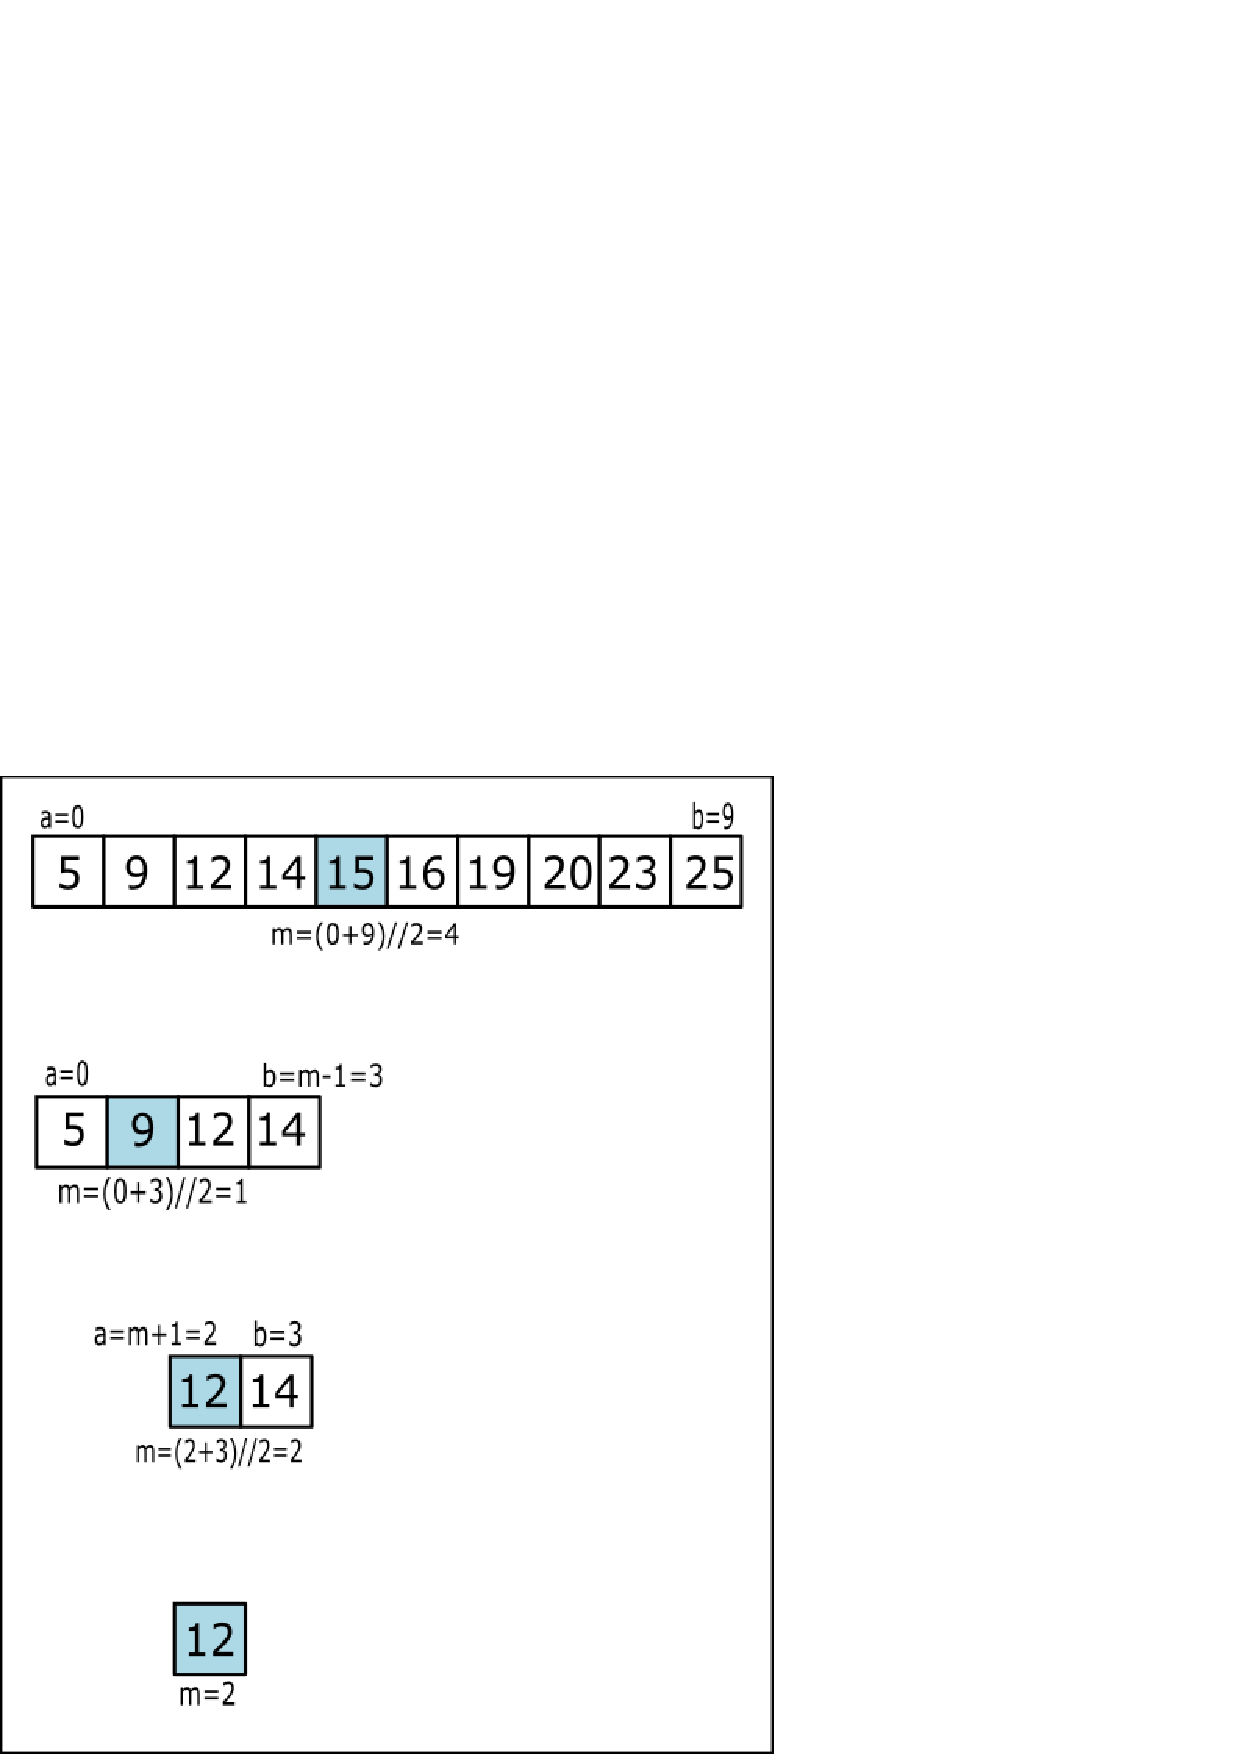
\includegraphics[scale=0.35]{../img/dichotomie.png}
\end{minipage}

\end{frame}


\begin{frame}
\frametitle{Recherche dichotomique}

\begin{exampleblock}{Exemple}
Si le nombre n'est pas présent dans le tableau, il faut que la boucle se termine! En voici les étapes avec la recherche du nombre $13$.
\begin{enumerate}
\item $a=0$ et $b=9$: $a<b$, donc on entre dans la boucle tant que.
\item On calcule $m=(0+9)/2=4,5$ donc $m=4$.

Comme $T[4]=15>13$, alors le nombre cherché est positionné avant $m$, donc $b=m-1=4-1=3$.

\item $a=0<b=3$, donc on poursuit la boucle: $m=(0+3)/2=1,5$ donc $m=1$.

Comme $T[1]=9<13$, alors le nombre cherché est positionné après $m$, donc $a=m+1=1+1=2$.
\item $a=2<b=3$, donc on poursuit la boucle: $m=(2+3)/2=2,5$ donc $m=2$.

Comme $T[2]=12<13$, alors le nombre cherché est positionné après $m$, donc $b=m-1=3-1=2$.

\item $a=2=b$ donc la boucle se poursuit: $m=(2+2)/2=2$.

$T[2]=12<13$, alors le nombre cherché est positionné après $m$, donc $b=m-1=2-1=1$.

\item $a=2>b=1$, la boucle s'arête, aucun nombre n'a été trouvé.
\end{enumerate}
\end{exampleblock}
\end{frame}

\begin{frame}
\frametitle{Terminaison de l'algorithme}

\begin{block}{Variant de boucle}
On appelle \textbf{variant de boucle} une quantité entière qui:
\begin{itemize}
\item doit être positive ou nulle pour rester dans la boucle;
\item décroit strictement à chaque itération
\end{itemize}
Si on trouve une telle quantité dans une boucle while, celle-ci se termine.
\end{block}

\begin{block}{Preuve de la terminaison}
Dans l'algorithme de recherche par dichotomie, le variant de boucle est $b-a$.
\begin{itemize}
\item Ce nombre est clairement supérieur ou égal à 0 puisque $a<=b$.
\item Vérifions qu'elle décroît en distinguant 3 cas:
\begin{enumerate}
\item[cas 1:] $t[m]==v$ alors on sort de la boucle.\medskip
\item[cas 2:] \begin{minipage}{6cm}
$t[m]>v$ donc $b'-a < m-a < b-a$ donc la quantité $b-a$ décroit.
\end{minipage}\hfill
\begin{minipage}{3.5cm}
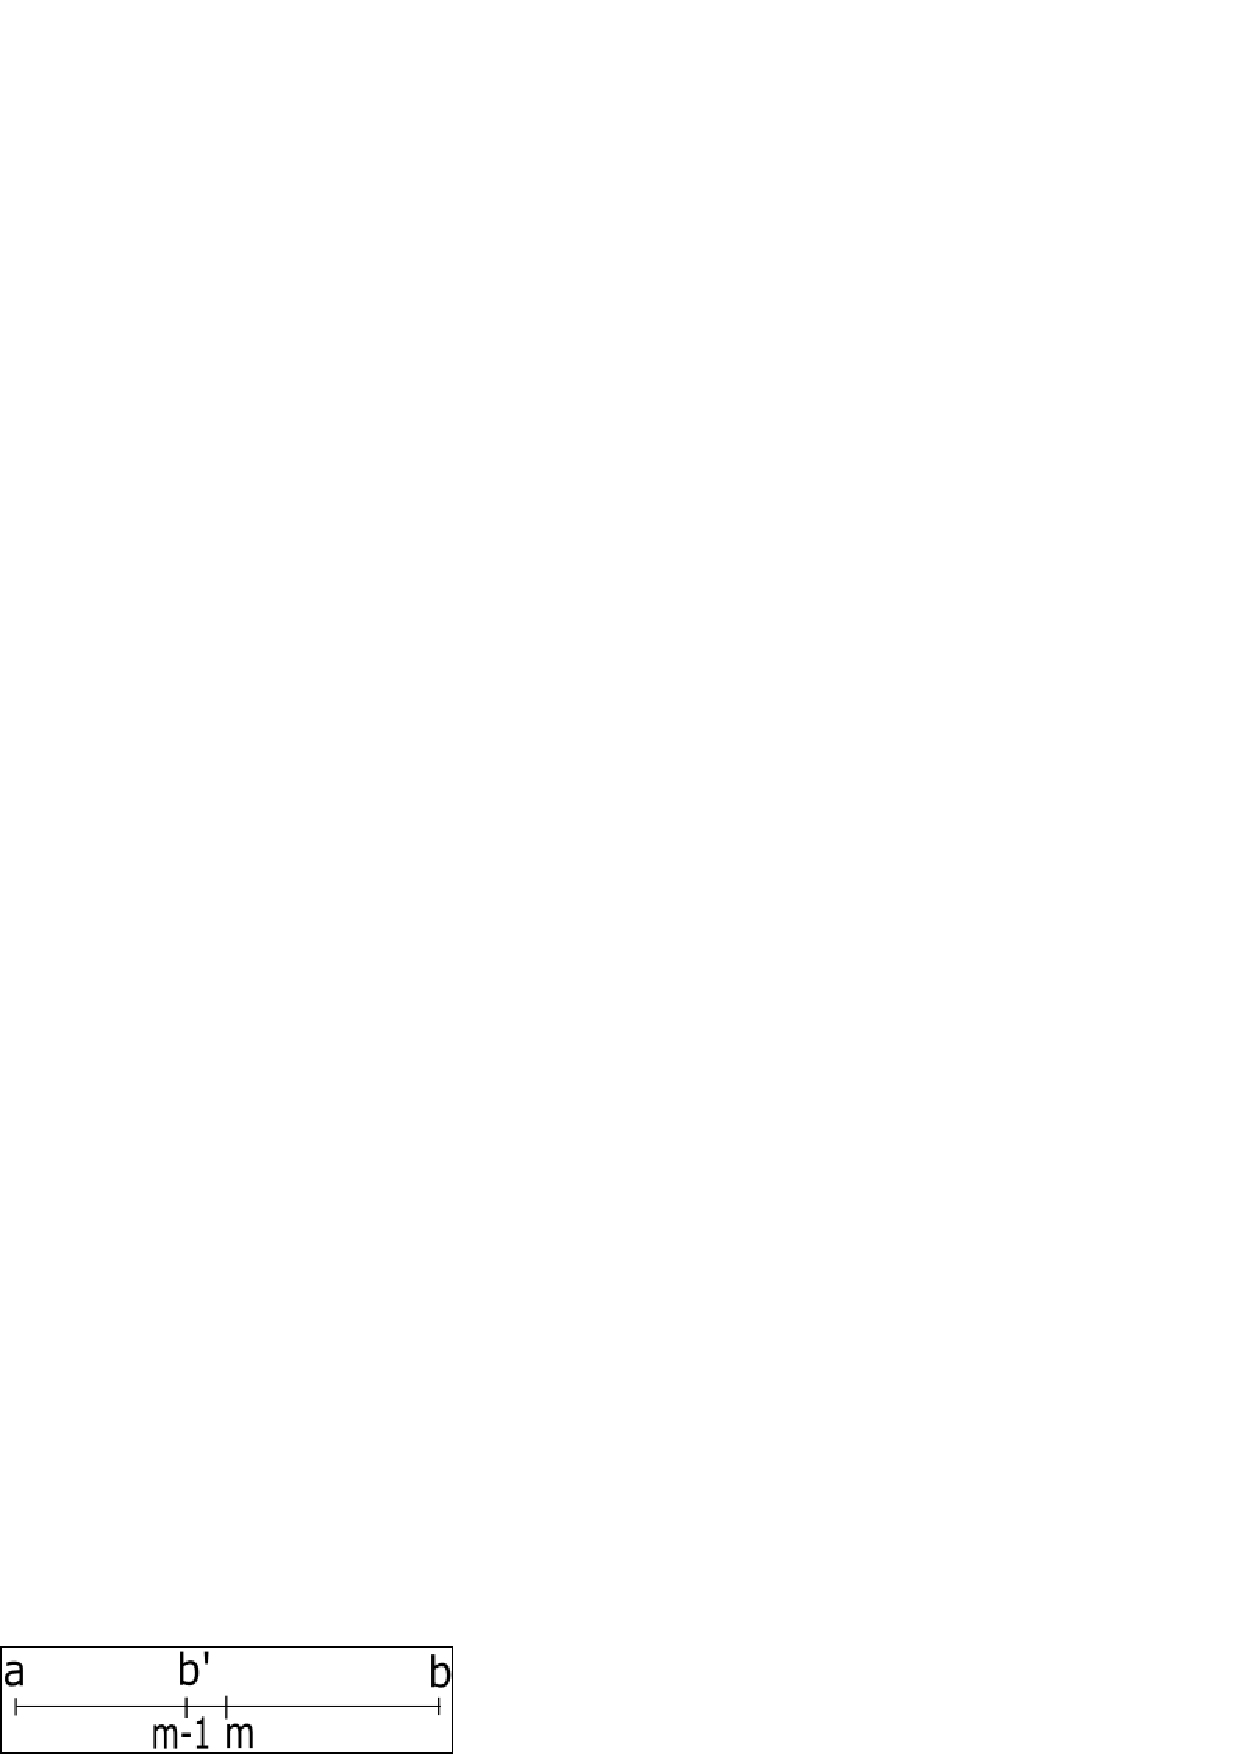
\includegraphics[scale=0.4]{../img/cas2.png}
\end{minipage}\medskip
\item[cas 3:] \begin{minipage}{6cm}
$t[m]<v$ donc $b-a' < b-m < b-a$ donc la quantité $b-a$ décroit.
\end{minipage}\hfill
\begin{minipage}{3.5cm}
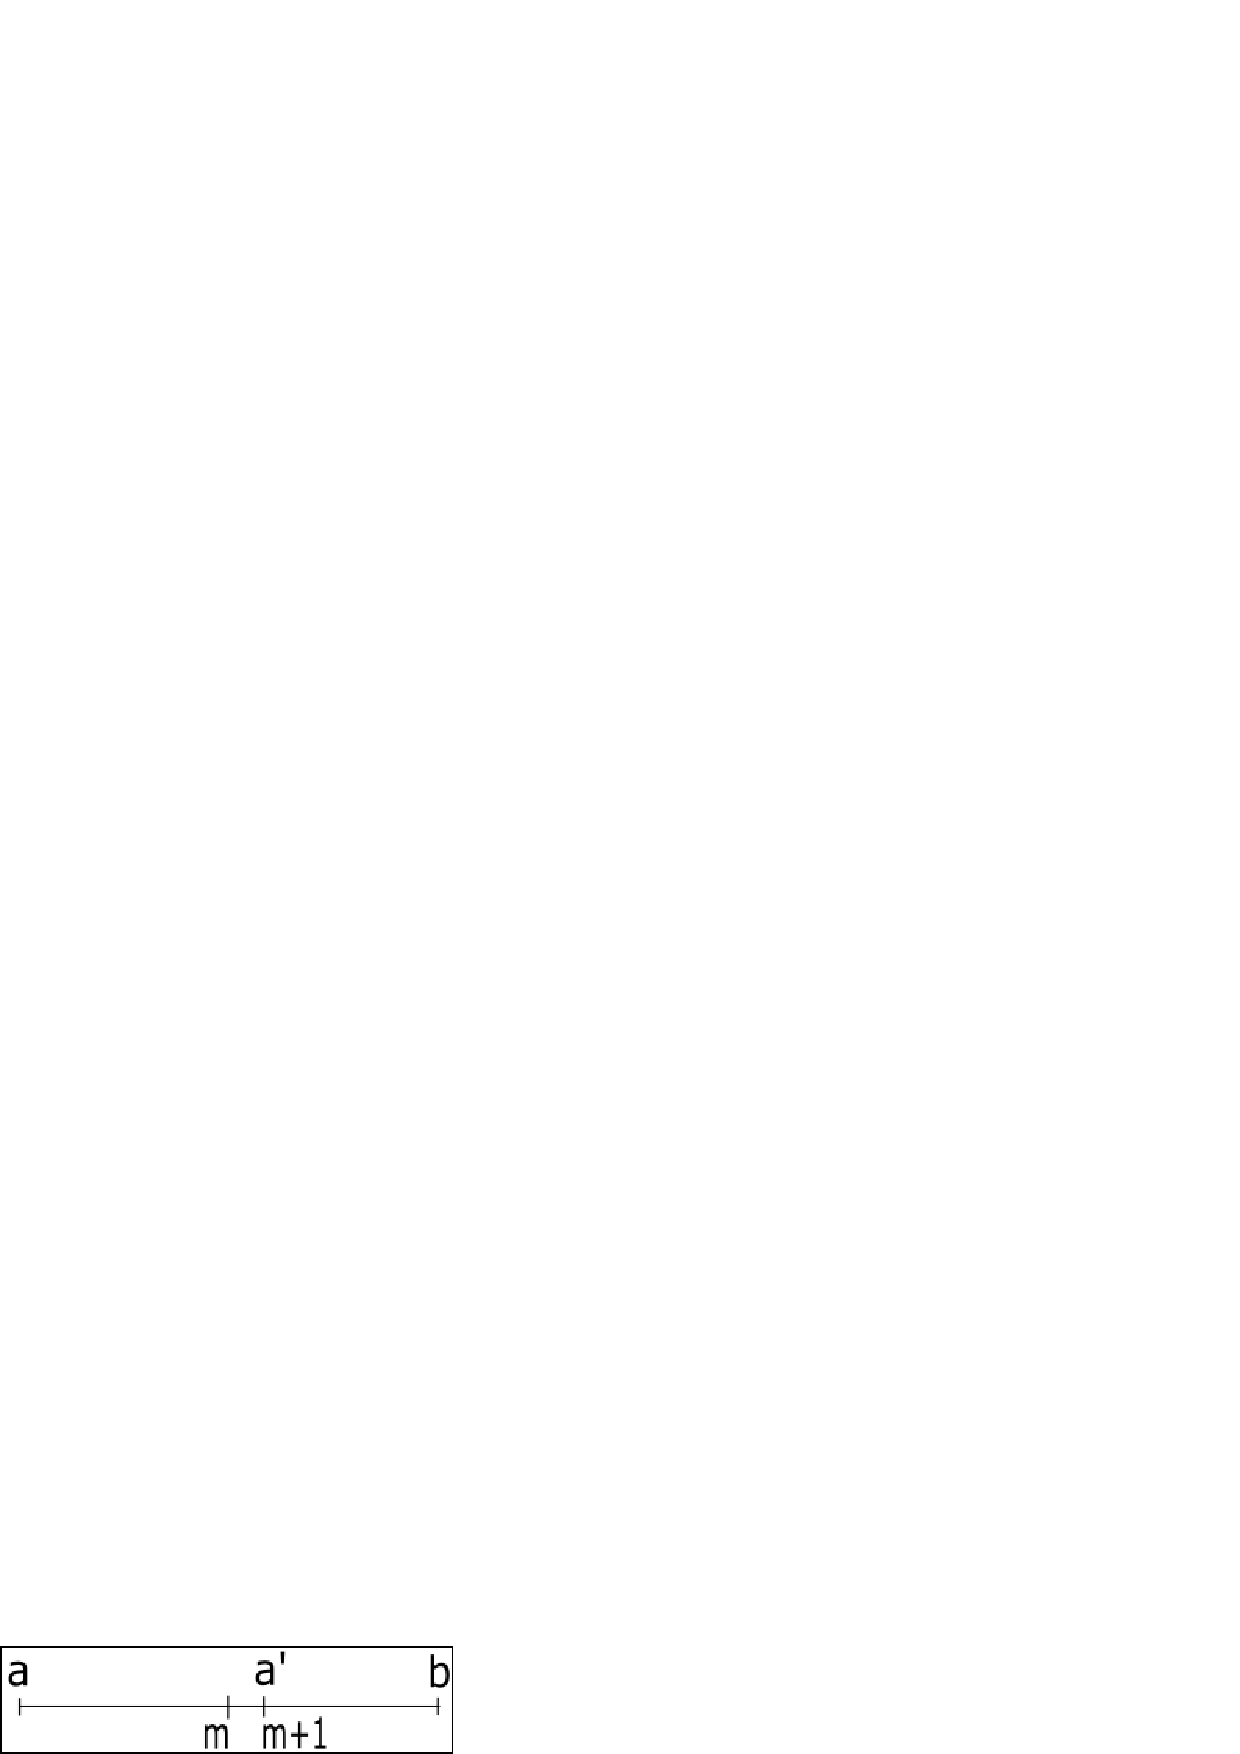
\includegraphics[scale=0.4]{../img/cas3.png}
\end{minipage}
\end{enumerate}
\end{itemize}
$b-a$ est un variant de boucle positif qui décroit, assurant la terminaison de la \textbf{boucle while}.
\end{block}
\end{frame}

\begin{frame}
\frametitle{Terminaison de l'algorithme}

\begin{exampleblock}{Exemple 1}
On cherche le nombre $12$ dans le tableau trié $T$. Les différentes valeurs de $a$ et $b$ sont:
\begin{enumerate}
\item $a=0$ et $b=9$ donc $b-a=9-0=\boxed{9}$
\item $a=0$ et $b=3$ donc $b-a=3-0=\boxed{3}$
\item $a=2$ et $b=3$ donc $b-a=3-2=\boxed{1}$
\end{enumerate}
La quantité $b-a$ est décroissante et positive tout le temps de la boucle.
\end{exampleblock}

\begin{exampleblock}{Exemple 2}
On cherche le nombre $13$ dans le tableau trié $T$. Les différentes valeurs de $a$ et $b$ sont:
\begin{enumerate}
\item $a=0$ et $b=9$ donc $b-a=9-0=\boxed{9}$
\item $a=0$ et $b=3$ donc $b-a=3-0=\boxed{3}$
\item $a=2$ et $b=3$ donc $b-a=3-2=\boxed{1}$
\item $a=2$ et $b=2$ donc $b-a=2-2=\boxed{0}$
\item $a=2$ et $b=1$ donc $b-a=1-2=\boxed{-1}$
\end{enumerate}
La quantité $b-a$ est décroissante, positive puis devient négative: on sort de la boucle.
\end{exampleblock}
\end{frame}

\begin{frame}
\frametitle{Coût, efficacité, complexité d'un algorithme}

\begin{block}{Introduction}
Déterminer l'efficacité d'un algorithme est important. Certaines instructions sons répétées de nombreuses fois et peuvent finir par prendre beaucoup de temps. On cherche alors à calculer un ordre de grandeur du nombre de calculs réalisés.
\begin{enumerate}
\item La recherche d'une valeur dans un tableau (minimum, maximum) est de complexité \textbf{linéaire}. Le nombre de calculs (comparaisons) est proportionnel à la dimension $n$ du tableau. On note cette complexité par $O(n)$.
\item Le tri d'un tableau par sélection ou insertion est de complexité \textbf{quadratique}. Le nombre d'opérations est proportionnel au carré de la dimension $n$ du tableau. On note cette complexité par $O(n^2)$.
\item La recherche par dichotomie est de complexité logarithmique. On la note $O(\log_{2}(n))$.
\end{enumerate}
\end{block}

\begin{block}{Propriété}
On peut comparer l'efficacité des algorithmes en comparant leur complexité. Pour un tableau de dimension $n$, on a: 
\[O(\log_{2}(n)) < O(n) < O(n^2)\]
\end{block}

\end{frame}
\end{document}

